\documentclass[12pt]{article}
\usepackage{graphicx}
\usepackage{amssymb}
\usepackage{epstopdf}
\usepackage{amsmath}
\usepackage{multicol}
\usepackage{tcolorbox}
\usepackage{geometry}
\usepackage{enumitem}
\usepackage{fancyhdr}

\DeclareGraphicsRule{.tif}{png}{.png}{`convert #1 `dirname #1`/`basename #1 .tif`.png}

\textwidth = 6.5 in
\textheight = 9 in
\oddsidemargin = 0.0 in
\evensidemargin = 0.0 in
\topmargin = -23pt
\headheight = 0.0 in
\headsep = 0.0 in
\parskip = 0.2in
\parindent = 0.0in
\pagestyle{fancy}
\pagenumbering{gobble}

\newtheorem{theorem}{Theorem}
\newtheorem{corollary}[theorem]{Corollary}
\newtheorem{definition}{Definition}
%\includegraphics [height=50mm, width=50mm]{PathInt.jpg}
\title{Title} 

\begin{document}
%INSTRUCTOR NOTES

 Name:
 \begin{center}\large{3.1 Derivatives of Polynomials}\end{center}

\textbf{Warm-up:} Put the following function in order: which is $f$, $f'$ and $f''$?\\
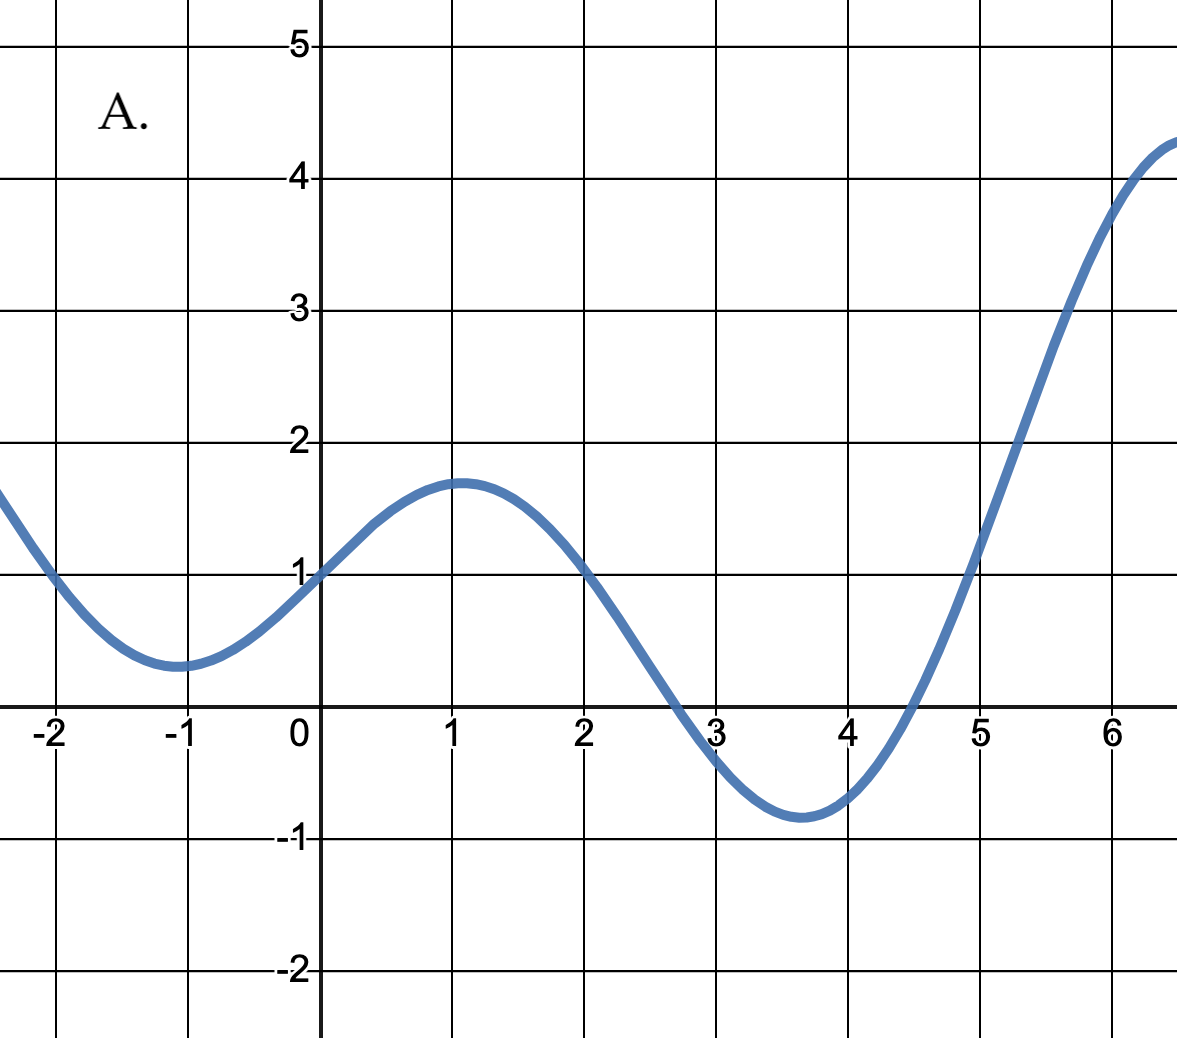
\includegraphics [scale=.12]{3_1_a}
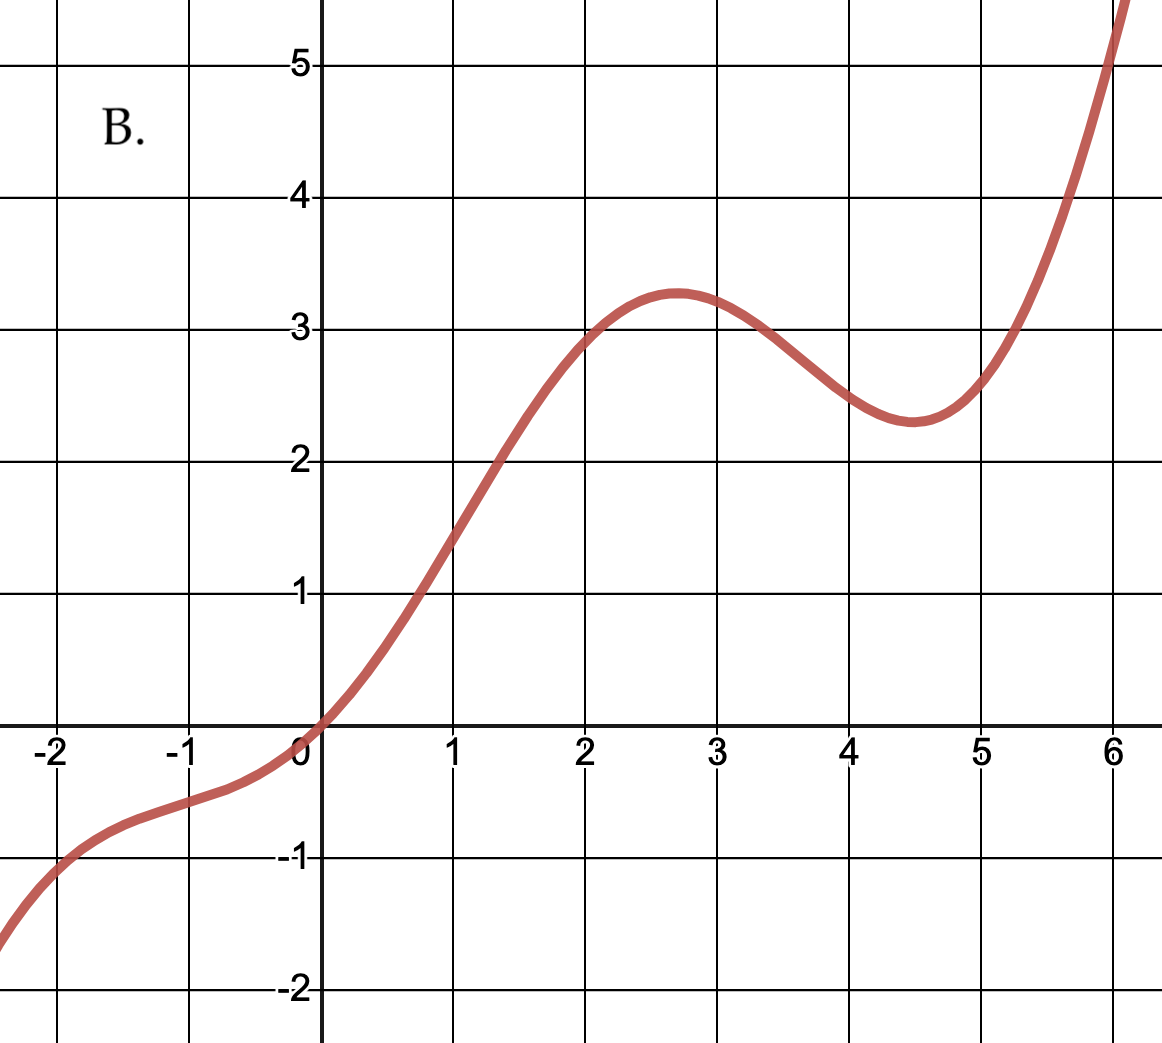
\includegraphics [scale=.12]{3_1_b}
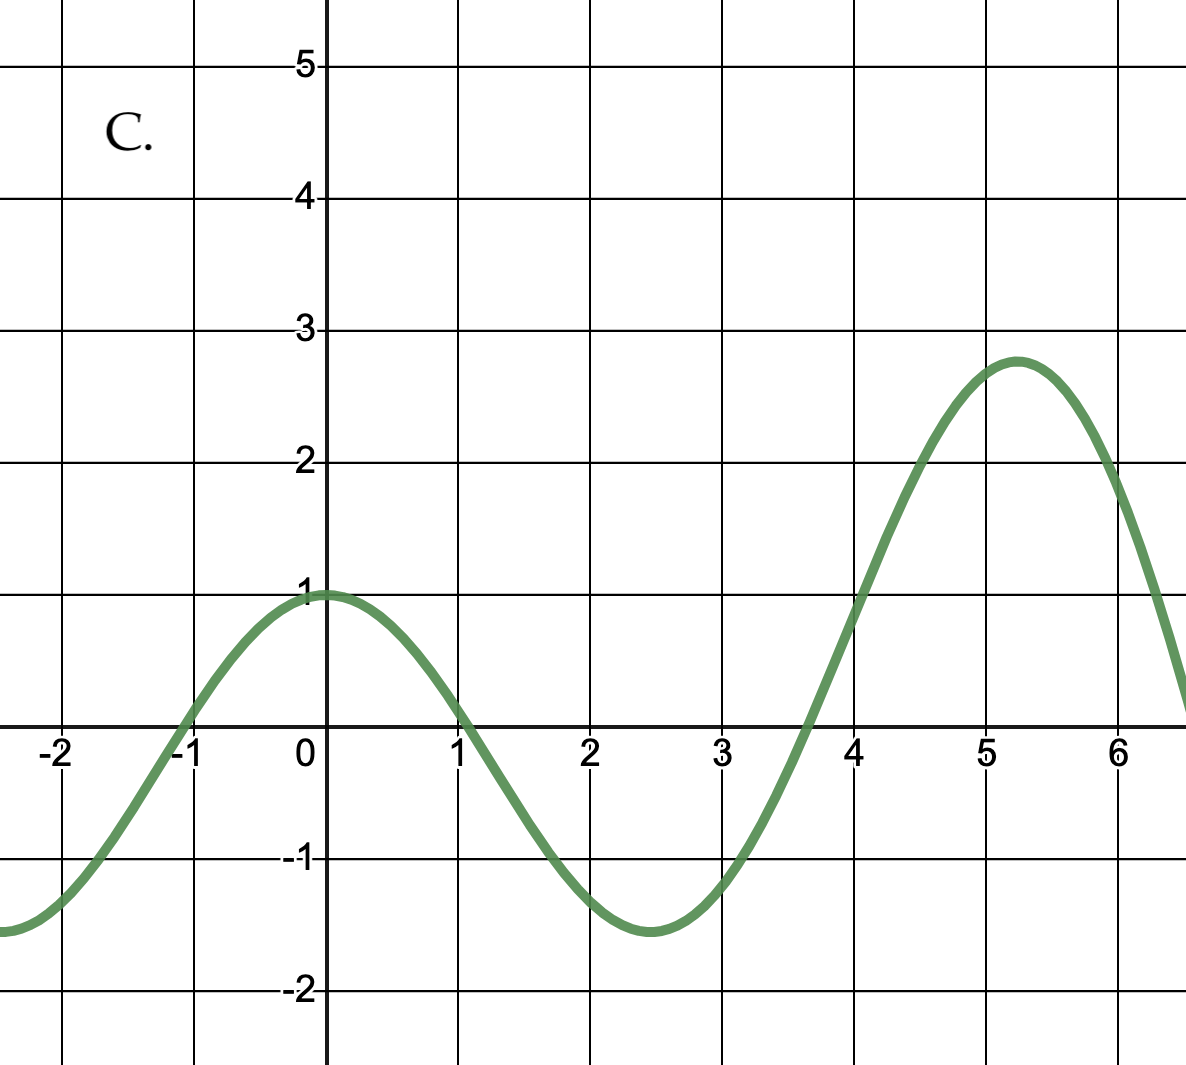
\includegraphics [scale=.12]{3_1_c}

\begin{enumerate}
\item Compute the following derivatives.
	\begin{enumerate}

	\item $k\left(x\right)=5x^{3}-2x+10$
	\vfill
	\item $g\left(s\right)=\sqrt{s}-2s^{\frac{2}{3}}$
		\vfill
	\item $f(x)=\pi^{2}-\frac{2}{x}$
		\vfill
	\item $h(t)=t^{3}(2t-5)$
		\vfill
	\end{enumerate}

\item Suppose $\displaystyle f\left(x\right)=x^{12}$. 
	\begin{enumerate}
	\item Find $\displaystyle\frac{d^{10}f}{dx^{10}}$. (Hint: look for a pattern!)
	\vfill
	\item Find $\displaystyle\frac{d^{14}f}{dx^{14}}$.
	\vfill
	\end{enumerate}
\newpage
~
\item If $M$ is the mass of the earth and $G$ is a constant, the acceleration due to gravity, $g$, at a distance $r$ from the center of the earth is given by

$$g=\frac{\left(GM\right)}{r^{2}}$$
	\begin{enumerate}
	\item Find $\displaystyle \frac{dg}{dr}$.
	\vfill
	\item What is the practical interpretation (in terms of acceleration) of $\displaystyle \frac{dg}{dr}$? Why would you expect it to be negative?
	\vfill
	\item You are told that $\displaystyle M=6·10^{24}$ and $\displaystyle G=6.67·10^{-20}$ where $M$ is in kilograms and $r$ in kilometers, and $g$ in km per sec$^{2}$. What is the value of $\displaystyle \frac{dg}{dr}$ at the surface of the earth ($r$ = 6400 km)? Include units.
	\vfill
	\item What does this tell you about whether or not it is reasonable to assume $g$ is constant near the surface of the earth?
		\vfill
 	\end{enumerate}
	
\item Find the equation of the line tangent to the graph of $f$ at $(1,1)$, where $f$ is given by $f(x)=2x^{3}-2x^{2}+1$. Check your work using Desmos.
	\vfill
\end{enumerate}	
\end{document} 

%%%%%%%%%
\begin{tcolorbox}
\textbf{Warm-up: } Solve the following equations for $t$.
\begin{multicols}{2}
\begin{enumerate}
\item $(t+1)^2=9$
\item $tx+x^2=5$
\end{enumerate}
\end{multicols}
\end{tcolorbox}

MINIPAGE
\noindent\begin{minipage}{0.3\textwidth}% adapt widths of minipages to your needs
try 1
\end{minipage}%
\hspace{40mm}
\begin{minipage}{0.6\textwidth}
a) $f'(2)=$\\\

b) $f'(4)=$\\

c) $f'(6)=$\\

d) $f'(7)=$\\

e) $f'(8)=$
\end{minipage}
